\subsection{Before asynchronism: discretization issues}

Here space discretization is taken as an a priori, while we discuss time and value discretization issues in this section.

\subsubsection{Time discretization issue}

Since symbolic resolution of differential equations such as (2) is not always possible, the evolution of the system can be approximated using numerical integration.

\paragraph*{A toy example}

\newcommand{\deq}{\stackrel {\rm def}{=}}

 Let us first consider the very simple case of a linear constant approximation of the system (2) with initial condition $V_j(0)$, in the particular case where leak $L_j$, connection strength $W_{jk0}$ and current input $I_j$ are constant, without transmission delays,
while $\sigma_j\left(u\right) = u$ (see \cite{Alexandre:2009} for a discussion of the kind of ``sigmoid'' profiles usually used). This writes in vectorial form:
$$\frac{\Delta V(t)}{\Delta t} = -{\bf W} \, {\bf V}(t) + {\bf I},$$
with
%%
\begin{align}
\label{eq:def-W}
{\bf W} \deq \left(\begin{array}{ccc} L_1 & -W_{120} & \cdots \\ -W_{210} & L_2 & \cdots \\  \cdots & \cdots & \cdots \\ \end{array} \right), \;
{\bf I} \deq \left(\begin{array}{c} I_1 \\ I_2 \\ \cdots \\ \end{array} \right),
\end{align}
%%
and its regular sampling forward Euler discretization writes: $ {\bf V}[i+1] = {\bf V}[i] - \Delta t \, {\Delta V(t)}\left/{\Delta t}\right.,$ at $t = i \Delta t$. 

Here, we have to assume that the system is contracting, i.e., that real part of the eigenvalues of ${\bf W}$ are strictly positive, otherwise the system does not converge towards a stable solution, and the Euler-forward approximation method is not expected to converge towards a continuous solution (see e.g. \cite{Press:1988} for these elementary notions).  In words this means that leak is strong enough with respect to the weights in order to induce the system convergence, see \cite{Alexandre:2009} for a detailed study in the case of discrete neural fields.  More precisely, on an eigendirection (i.e. in the direction of an eigenvector of the matrix), the linear equation is decoupled from the others and the leak (either a real or a complex value) corresponds to the opposite of the eigenvalue, with solution either as damped oscillations or as an exponential vanishing profile.  We do not have to assume that weights are symmetric, but that the matrix ${\bf W}$ is diagonalizable, which is always the case up to a negligible singular set, not taken into account here.
%%
\begin{figure}[!htbp]
\begin{center}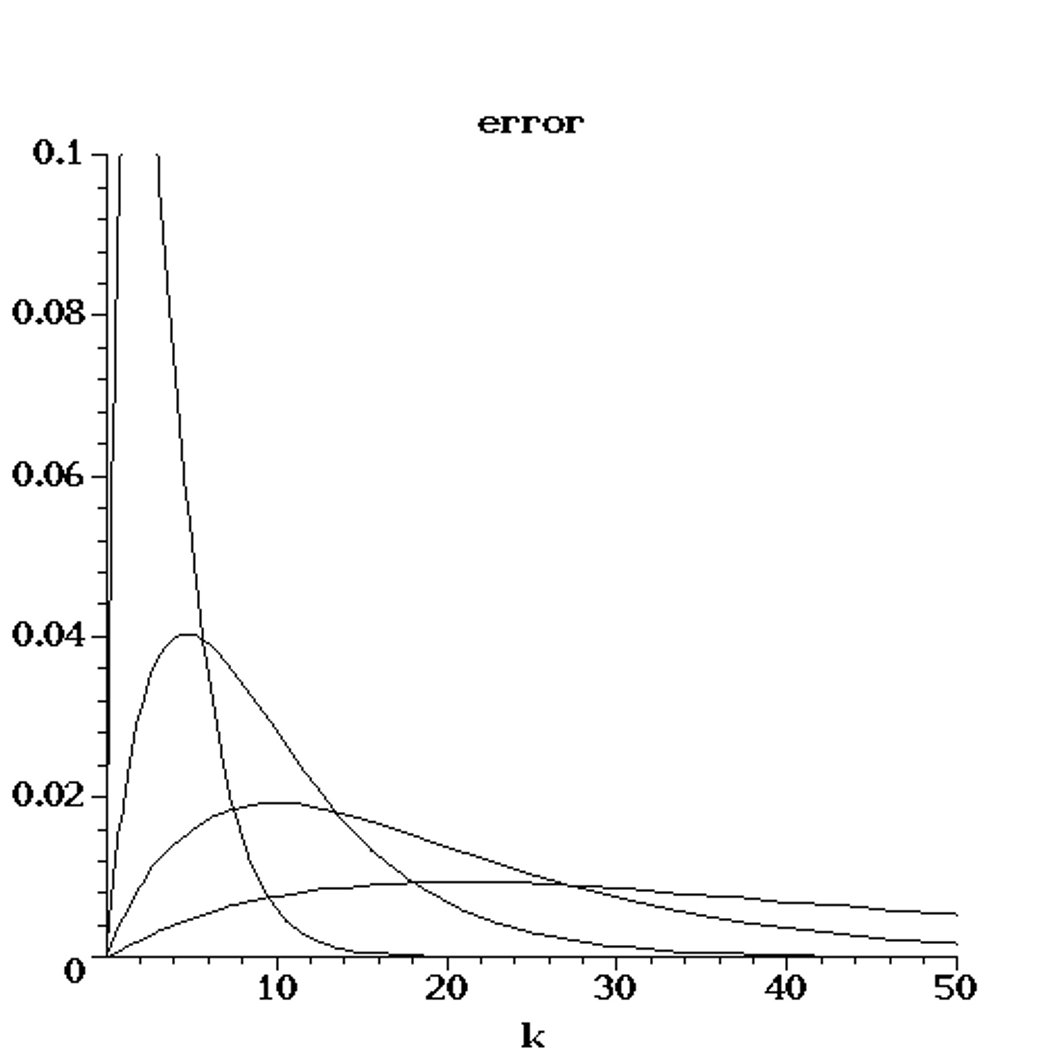
\includegraphics[width=0.25\textwidth]{Chapitres/PublicationsSample/Revue/fig1a.jpeg}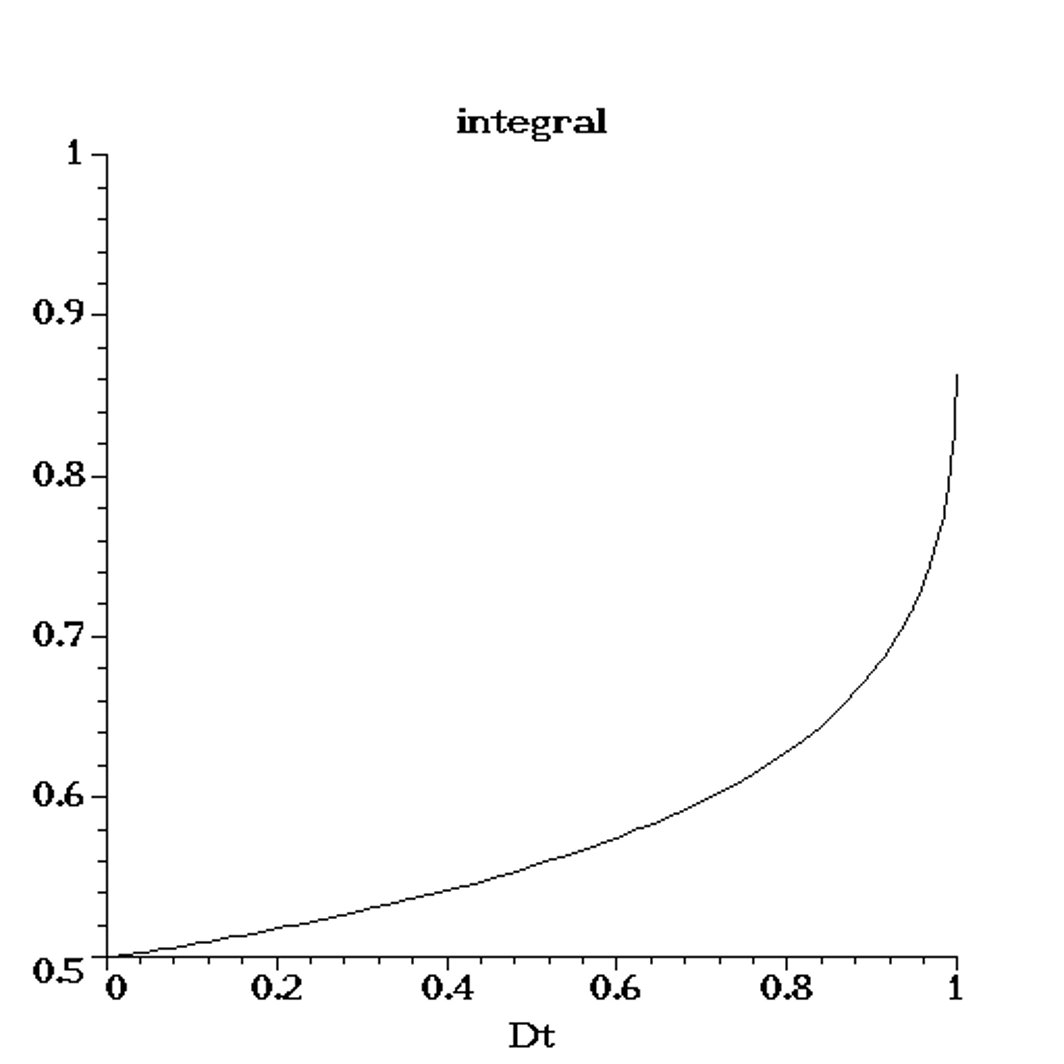
\includegraphics[width=0.25\textwidth]{Chapitres/PublicationsSample/Revue/fig1b.jpeg}\end{center}
\caption{{\em Left view}: The normalized bias temporal profile between the continuous scheme and its discrete approximation,
drawn here for $\Delta t / \tau_j = [0.05, 0.1, 0.2, 0.5]$ from the flattest to the sharpest curve respectively.
{\em Right view}: The integral of the bias along the trajectory as a function of $\Delta t / \tau_j$, making explicit that the cumulative bias is never negligible even for very small leak, while it diverges for large leak.
See text for details.}
\label{fig:euler-error} 
\end{figure} 
%%
In such a simple case,\footnote{In the scalar case, an explicit closed-form is automatically derived from a few lines of, e.g., {\tt maple} symbolic code:
\\{\tiny \tt \begin{tabular}{l}
eq := D(V)(t) = -W * V(t) + b: assume(0 < W, W < 1): \\
\# Continuous solution, assuming t0 = 0 \\
s\_c := dsolve({eq, V(0) = V0}, V(t)); \\
\# Euler approximate integration, assuming delta\_t = 1 \\
s\_e := rsolve({subs(eq, t = k, V(k + 1) = V(k) + Dt * D(V)(t)), V(0) = V0}, {V}); \\
\# Bias analysis \\
err\_k := simplify(factor((subs(s\_c, t = Dt * k, V(t)) \\
- subs(s\_e, V(k))) / (V0 - i / W)), {Dt * W = c}); \\
\end{tabular}}\\ while the result is straightforward to apply to the eigenvalue decomposition of the ${\bf W}$ matrix.
Furthermore, in the scalar case, 
if the Euler approximation is used with $Dt = (1 - exp(-W \, \Delta t)) / W = \Delta t - W/2 \Delta t^2 + O(\Delta t^2 )$ in numerical scheme,
the bias is canceled, which is not generalizable in the vectorial case since it depends on the leak value.
}
%%
both the continuous scheme and its discrete approximation starting from the same initial value converge towards the same fixed point (which can be found in all textbooks), but not though the same trajectory (which is surprisingly not studied in text books up to our best knowledge).  More precisely the bias in an eigendirection of the ${\bf W}$ matrix is proportional to $V_j(0) - I_j \, \tau_j$, where $1/\tau_j$ is the eigenvalue (i.e., the leak) in this direction, and follows a double exponential profile, only function of $\Delta t / \tau_j$, as illustrated in Fig.~\ref{fig:euler-error}. In words, the higher $\Delta t / \tau_j \in [0, 1[$ (this boundaries corresponding to the convergence interval), the higher the bias magnitude, but the quicker the bias between both methods vanishes.  The highest leak thus determines the maximal bias, the smallest leak the maximal duration of bias. \\

It is a counter-intuitive and very important result to notice that large leaks (i.e. small time-constants) indeed accelerate convergence, but with the drawback to generate large errors during the first iterations.  This means that the system dynamics may very easily switch from one attractor to another, at the beginning of the trajectory, even in such a very simple case.

\paragraph*{The general case: consequences}

In more general cases, there is no cute closed-form formula, as in the previous toy example, but it is obvious to infer to which extends the same kind of bias occurs.

In the non-constant case (i.e., leak, weights or currents vary with time), the previous results generalize considering bounds of the, now variable, leaks. 
In the non-linear case, the previous results generalize bounding the non-linear function $\sigma_j()$ by the corresponding maximal slope linear function.
See, e.g. \cite{Cessac:2007} for a review of such tools.
More precisely, if the system is hyperbolic, the same condition applies on the Jacobian of the system at any time and state value.

If the input variable $I_i(t)$ is not constant, we are thus in the situation where we track the true solution, and this is qualitatively equivalent to be reset at a new initial state at each step. As a consequence for small $\Delta t / \tau_j$ the system is expected to be always in a transient biased state with first iteration large errors, whereas for large  $\Delta t / \tau_j$ the system is always going to have a non-negligible lag with respect to the true solution. There is clearly a trade-off to find out, but always impaired by an incompressible bias.

As a consequence, we learn something from the present tiny analysis, even in more general cases: the method never converges at the trajectory level.
In any case, the cumulative bias is never negligible, with a lower bound for small leak, while diverging for large leaks.
This shows the very important difference between the fact that the discretization methods {\em converge at least} toward the expected fixed point 
and the fact that the simulation trajectory is unbiased. In the toy example, unbiasness never occurs, except in the singular case where $V_j(0) = I_j \, \tau_j$. Where stands the ``mistake'' ? At the implementation level, it stands on the simple fact that we are stick to synchronous computations.

\paragraph*{When asynchronism solves the situation}

At the implementation level, we obviously need several sampling times for a given simulation time in order to make the discrete approximation converge towards the continuous one,
which is often not taken into consideration. 

At the modeling level, the present mistake stands on the belief that a pertinent model of the reality has to be a ``continuous'' model, its discretization being a kind of second-class implementation detail. 
This is definitely wrong when modeling digital computational systems, but this is also questionable for microscopic neural models 
(see, e.g., \cite{Cessac:2008} for a discussion on biologically plausible generalized integrate and fire neuron models)
and mesoscopic neural map models (see, e.g. \cite{Rougier:2006} for a discussion at this modeling scale), 
the key question being ``what do we want to learn'' from the model or its simulation.

Now let us reconsider equation~(\ref{eq:DNF-discrete}) in the asynchronous computation paradigm. We have at time $t$, estimations of other units $\{\hat{V}_j(t)\}$, and estimations of the input $\hat{I}_i(t)$, and have missing values specified as a first approximation, as discussed in section~\ref{paradigm}. We thus can approximate:
%%
\begin{align}
\hat{J}_i(t) = \hat{I}_i(t) + \sum_{\substack{j \in M\\k \in \{k_{\min}, k_{\max}\}}} W_{ijk} \, \sigma_j\left(\hat{V}_j(t - k\, \Delta T)\right) \notag
\end{align}
%%
and are left with solving:
%%
\begin{align}
\frac{\Delta V_i(t) }{\Delta t}  = - L_i \, V_i(t)  + \hat{J}_i(t) \notag
\end{align}
%%
with the obvious closed form solution:
%%
\begin{align}
\label{eq:DNF-solution}
\hat{V}_i(t) = V_i(0) \, e^{-L_i t} + \int_0^t d\eta \, e^{-L_i (t - \eta)} \, \hat{J}_i(\eta)
\end{align}
%%
which is straightforward to iteratively approximate up to some adjustable time $t$, at any degree of precision, and easy to update as soon as better estimations of $\hat{J}_i(t)$ are available. Several further implementation choices are to be specified up to this point, but it is clear that all ingredients are there to design an asynchronous implementation of~(\ref{eq:DNF-discrete}).

\subsubsection{Value discretization issues}\label{dds}

A Discrete Dynamic System (DDS) is a finite set of elements, each taking a finite number of states evolving in a discrete time, by mutual interactions. In \cite {Robert:1994}, a book dedicated to the analysis of the temporal dynamics of such systems, Robert proposes a general framework, i.e., "a chaotic discrete iteration mode", to analyze such systems. The studied system is a cellular automaton with $N$ Boolean cells (a finite number of states), which may correspond, in a neural network, to an active neuron state (spiking) or a silent state. Each unit\footnote{More precisely, starting from an initial state at $t=0$, at each time step each unit updates its state function involving the states of the corresponding subset of elements, using any specific iteration mode (parallel, serial or chaotic).} is influenced by a subset of units that are involved in its update. 

Indeed, though a computer variable takes a finite number of values, the DDS results do not apply to floating-point number representations, because the order of magnitudes of the results are not usable in practice. Furthermore, DDS are not sufficient for modeling the targeted systems, i.e. DNF, that represent physical quantities, thus are best modeled by differential equations with continuous values. However, depending on the level of modeling, DDS could encounter for qualitative behaviors and we include them in the discussion in the sequel.

